%-------------------------------------------------------------------------------
\chapter{R\'esum\'e}
\labelchapter{ch.resume}
%-------------------------------------------------------------------------------

%%%%%%%%%%%%%%%%%%%%%%%%%%%%%%%%%%%%%%%%%%%%%%%%%%%%%%%%%%%%%%%%%%%%%%%%%%%%%%%%
%%%%%%%%%%%%%%%%%%%%%%%%%%%%%%%%%%%%%%%%%%%%%%%%%%%%%%%%%%%%%%%%%%%%%%%%%%%%%%%%

\lettrine[lines=2]{C}{e} chapitre propose un bref résumé du contenu de ce manuscrit, en français.
Il s'agit d'une synthèse du travail qui a été effectué durant cette thèse, et qui est décrit en anglais dans les chapitres précédents.

Ce résumé commence par un exposé des motivations à l'origine de ces travaux, et présente ensuite les travaux existants dans l'état de l'art quand au domaine de l'exploration d'espace de conception.
Les deux sections suivantes concernent les contributions de cette thèse, respectivement la définition et l'estimation de métriques d'intérêts pour la conception numérique, et une méthodologie novatrice d'exploration d'espace de conception basée sur l'utilisation des langages de construction matérielle, à savoir la {\bf méta exploration}.
Ensuite, les expérimentations qui ont été menées pour démontrer l'utilisabilité des méthodologies proposées sont présentées, conjointement avec un démonstrateur logiciel spécialement développé pour cette thèse, nommé {\it Quick Exploration using Chisel Estimators} ({\bf QECE}).
Finalement, une synthèse sur les contributions de cette thèse est proposée, et les limitations de ces travaux sont mises en avant afin demettre l'accent sur les pistes de recherches qui restent ouvertes à la fin de cette thèse.

\vspace*{\fill}
\minitoc 
\mtcskip 

\newpage
%%%%%%%%%%%%%%%%%%%%%%%%%%%%%%%%%%%%%%%%%%%%%%%%%%%%%%%%%%%%%%%%%%%%%%%%%%%%%%%%

\section{Motivations}
\label{ch.resume:sec.motivations}
    Les motivations qui se cachent derrière ce travail de thèse sont à contextualiser par rapport à l'évolution historique des flots de conception numérique.
    En effet, les méthodologies de conception de circuit ont drastiquement évoluées au cours des dernières décennies, des méthodes de dessin de masque jusqu'aux techniques de synthèse de haut niveau qui sont désormais utilisées dans l'industrie.

    Cependant, les alternatives actuelles qui s'offrent aux développeurs reposent soit sur des langages de description matérielle, comme VHDL ou Verilog, et requièrent un niveau d'expertise ainsi qu'un temps de développement conséquent, ou sur des méthodologies qui impactent les performances des circuits conçus, comme la synthèse de haut niveau ou les langages à domaine spécifique.

    Dans ce contexte, nous nous sommes intéressés à l'utilisation d'un paradigme de développement matérielle qui a récemment vu le jour : les langages de construction matérielle, qui, comme leur nom l'indiquent, proposent une approche plus constructiviste de la conception numérique.
    Se faisant, ces langages permettent de décrire des générateurs de circuits plutôt que des circuits dont la fonctionnalité et les possibilités sont figées à la conception.

    Plus particulièrement, nous proposons dans ce travail d'étudier l'utilisation de ces langages dans le contexte de l'exploration d'espace de conception, c'est à dire le processus --- manuel, assisté ou automatique --- qui consiste à faire varier des architectures équivalentes en terme de fonctionnalité, afin de les comparer entre elles et de sélectionner celle qui répond le mieux à un cas d'utilisation donné.

    Les fonctionnalités de génération propres aux langages de construction matérielle se trouvent donc être une opportunité intéressante pour proposer des flots d'exploration d'espace de conception qui, contrairement à leurs équivalents de plus haut niveau (notamment ceux utilisés dans les techniques de synthèse de haut niveau), permettent aux développeurs de contrôler les circuits générés tout en guidant, à l'aide de leurs expertises, les outils pour converger rapidement vers une solution adaptée au cas d'utilisation initial.

\section{État de l'art}
\label{ch.resume:sec.state}
    Afin de positionner nos travaux par rapport à la littérature existante dans le domaine de l'exploration d'espace de conception, nous nous proposons d'analyser les différents outils et méthodologies d'exploration sous trois angles : l'exposition de l'espace à explorer, les métriques d'intérêt à considérer pour estimer la "qualité" d'une implémentation en particulier, et la façon dont les architectures en jeu sont comparées entre elles afin de sélectionner la ou les meilleure(s) solution(s).

    L'exposition de l'espace de conception est un point clef pour définir des processus efficaces d'exploration.
    En effet, si l'espace considéré inclut trop de solutions, notamment des solutions qui sont trivialement sous optimales (comme cela peut être le cas si un outil est utilisé pour générer un tel espace), le processus d'exploration sera peu efficace, car il devra comparer trop d'architectures différentes (chaque comparaison pouvant s'avérer très coûteuse).
    D'un autre côté, si l'espace considéré est trop restreint, le développeur risque de ne pas considérer une solution qui serait "meilleure" que celles qu'il a étudiée, pour un cas d'utilisation donnée.
    Ainsi, les approches d'exposition d'espace existantes se positionnent sur un spectre continu de solutions, qui va d'espaces composés de variations qui sont toutes manuellement définies par le développeur (qui contrôlent donc totalement les circuits qui sont considérés) à des espaces où l'ensemble de ces variations est inféré par un outil de façon implicite (par exemple, dans le cas de la synthèse de haut niveau, les outils décident eux mêmes de comment les différentes primitives de programmation logicielle seront traduits dans le paradigme de description matérielle).
    La plupart des solutions existantes se situent en réalité quelque part sur ce spectre, et combinent donc des paramètres explicites pour contrôler les variations fines d'architecture, afin d'optimiser la performance des circuits générés, et des inférences implicites qui permettent aux développeurs de ne pas s'attarder sur certains aspects simples des circuits pour lesquels les heuristiques d'inférence fonctionnent bien.
    On notera ici la nécessité pour le développeur de pouvoir intervenir dans le processus d'exposition d'espace de conception, afin de pouvoir s'il le souhaite proposer des variations qui lui semblent pertinentes pour améliorer la qualité des architectures proposées, mais aussi le processus d'exploration en lui même (par exemple en supprimant certaines inférences si elle ne semblent pas intéressantes).%
    \footnote{Cette philosophie --- s'appuyer sur l'expertise des développeurs et développeuses matériels pour améliorer leurs productivités --- est d'ailleurs à la base de ces travaux, qui cherchent à proposer un flot de conception totalement personnalisable qui permette à ces utilisateurs de contrôler les aspects de conception qui leur semblent importants tout en reposant sur de simples inférences pour les décharger des tâches les plus simples et ainsi améliorer leurs expériences de conception.}

    Une fois l'espace de conception défini pour un cas d'utilisation donné, le développeur doit définir les métriques d'intérêts, ainsi que les méthodologies d'estimation adéquates.
    Ce faisant, il fournit en réalité les bases de fonctions objectifs à optimiser, en spécifiant une façon de mesurer la qualité des architectures de façon automatique.
    Ces métriques sont, pour les plus usuelles d'entre elles, omniprésentes dans le travail quotidien des développeurs --- il peut s'agir de l'utilisation des ressources disponibles, de la fréquence d'opération ou encore de la bande passante utilisée par les architectures considérées.
    Nous proposons également de considérer des métriques plus "exotiques", comme la qualité de résultat (qui peut se définir, par exemple, par le taux d'erreur induit sur les résultats d'un circuit par rapport à une référence) ou encore la durée de vie des variables ou la sécurité des architectures.
    L'accent est particulièrement mis, encore une fois, sur l'intérêt qu'ont les développeurs à pouvoir définir eux même à la fois les métriques considérées, mais aussi les techniques pour estimer ces métriques, ce qui peut notamment influer sur la précision de ces estimations et sur leur rapidité.

    Enfin, nous proposons de considérer un dernier aspect clef dans la définition de méthodologies d'exploration d'espace de conception : la stratégie d'exploration.
    Cette stratégie désigne l'algorithme qui va être utilisé lors du procédé d'exploration afin de comparer les différentes implémentation entre elles, cet algorithme étant le plus souvent implémenté dans l'outil d'exploration, mais correspond également au processus d'optimisation bien connu des concepteurs numériques, qui le plus souvent itèrent sur la description matérielle jusqu'à obtenir une solution qui satisfassent leurs contraintes et objectifs.
    Pour ce troisième point, nous appuyons notre analyse sur différentes taxonomies de stratégie d'exploration existantes dans la littérature.
    Tout d'abord, nous considérons trois types de stratégie possible pour explorer un espace de conception : les stratégies hiérarchiques, les stratégies itératives et les stratégies séquentielles.
    Bien que les stratégies hiérarchiques et itératives semblent très prometteuses dans le domaine de l'exploration, notamment pour leurs capacités de passage à l'échelle, nous nous sommes concentrés sur les stratégies séquentielles dans le cadre de ces travaux, c'est à dire des algorithmes qui s'appuient sur un ensemble d'étapes consécutives qui opèrent sur l'espace de conception afin de répondre à un cas d'utilisation.
    La deuxième taxonomie considérée dans cette approche classifie ces algorithmes en quatre catégories : les méta-heuristiques, les heuristiques dédiées, les méthodes basées sur l'apprentissage supervisé et les méthodes basées sur des analyses de graphe.
    Ces différentes catégories mettent en avant l'immense variété de possibilité qui s'offrent au développeur qui souhaite explorer de façon efficace son espace de conception, et appuient une fois de plus notre proposition de méthodologie générique et flexible reposant sur les connaissances et l'expertise du développeur pour guider le processus d'exploration.

    \clearpage

    Dans cette analyse de la littérature, nous montrons donc que le domaine de l'exploration d'espace de conception est un domaine très vaste, qui comporte de nombreuses contributions et méthodologies.
    Cependant, l'analyse de l'état de l'art en trois point qui est proposée est, au vue de nos connaissances actuelles, novatrice dans son approche du problème d'exploration, ces considérations d'exposition, d'estimation et d'exploration n'étant usuellement pas décorrélées mais plutôt considérées comme un tout.
    De plus, cette analyse met en avant l'intérêt d'une méthodologie d'exploration qui soit flexible et basée sur l'expérience des développeurs, là où la plupart des initiatives actuelles cherchent plutôt à permettre à des utilisateurs non experts de réaliser cette tâche d'exploration, et ce le plus souvent au coût de la performance des circuits générés.

\section{Métriques et méthodologies d'estimation}
\label{ch.resume:sec.estimation}
    Dans ce chapitre, nous explicitons l'intérêt de la tâche de définition des métriques d'intérêt dans le cadre de l'exploration d'espace de conception.
    En effet, il est nécessaire de définir une sorte de relation d'ordre entre les différentes implémentations qui composent cette espace : factuellement, cela revient à expliciter les critères de qualité qui sont à considérer pour définir si une implémentation est préférable à une autre dans le cas d'utilisation donné.

    Il est à noter que cette étape de définition explicite des métriques d'intérêt s'intègre encore une fois dans notre approche flexible du problème de l'exploration d'espace de conception : dans la plupart des outils, ces métriques sont au mieux définies "en dur" dans les outils (et l'utilisateur peut choisir laquelle il souhaite considérer), et au pire ne sont même pas paramétrables.
    A contrario, nous faisons le choix dans ce travail de laisser au développeur la liberté de définir les métriques d'intérêts pour son cas d'utilisation, mais aussi de définir les méthodologies d'estimation qui seront utilisées pour définir ces métriques.

    En effet, après avoir défini une métrique de qualité pour les implémentations qui composent l'espace à explorer, il est nécessaire de préciser comment cette métrique doit être calculée : cela peut être par des formules analytiques, des analyses de la représentation interne du circuit dans le flot de compilation Chisel, ou encore l'interfaçage avec des outils externes.
    Par exemple, pour estimer la consommation de ressources d'une implémentation, on peut décider d'utiliser une simple estimation (rapide) basée sur le comptage des primitives de calcul qui apparaissent dans la représentation du circuit, mais on peut aussi utiliser les résultats d'un outil de synthèse logique (bien plus long, mais bien plus précis) afin de fournir à l'outil d'exploration des métriques plus réalistes.
    Ainsi, nous proposons une méthodologie générique à la fois de définition et d'estimation des métriques d'intérêt, qui s'appuie sur une interface de programmation flexible qui permet d'intégrer ces estimateurs à différents niveaux d'abstraction, en jouant sur un compromis implicite entre la qualité d'un estimateur et sa rapidité.

    Nous proposons également dans ce chapitre l'implémentation de plusieurs estimateurs comme autant de preuves de concept de l'utilisabilité de cette approche.
    Nous implémentons ainsi tout d'abord un estimateur rapide de la consommation de ressource FPGA, basé sur une analyse hiérarchique de la représentation intermédiaires des circuits générés par Chisel.
    Un estimateur similaire pour le calcul des chemins critiques des circuits est proposé, mais la difficulté de l'approche ainsi que sa complexité algorithmique résultent en une solution qui est à la fois trop imprécise et trop lente pour être utilisable en pratique.
    Afin de fournir des estimations réalistes, nous proposons une interface simple pour les logiciels de synthèse logique propriétaire, permettant d'estimer à la fois la consommation de ressources et les chemins critiques d'un circuit.
    Cette estimateur est donc relativement lent, mais très utile dans la mesure où les résultats de ces outils de synthèses devront être considérés tôt ou tard dans le processus de conception d'un circuit.
    Enfin, nous implémentons un estimateur plus original, qui consiste à estimer la qualité de service des différents circuits générés.
    Cette métrique d'intérêt, qui peut s'avérer cruciale dans des domaines tel que celui des calculs approximés, est rarement considérée dans les flots d'exploration classique, et cette proposition permet de démontrer l'intérêt de la définition de métriques personnalisées par le développeur, pour des cas d'utilisation très particuliers.
    L'estimation de la qualité de service est basée sur deux approches distinctes : le développeur peut fournir un modèle analytique pour estimer le taux d'erreur introduit dans le circuit par rapport à ses paramètres de génération, ou peut utiliser une approche empirique, basée sur les résultats de simulations RTL des circuits, afin d'estimer ce même taux d'erreur.

    Dans ce chapitre, nous proposons donc à la fois une approche générique pour la définition et l'estimation de métriques d'intérêt dans le contexte de l'exploration d'espace de conception, mais aussi des estimateurs "preuves de concept" qui s'intègrent dans le flot de conception Chisel à travers l'interface de programmation que nous avons définie.

\vspace{-0.27cm}
\section{Exploration d'espace de conception}
\label{ch.resume:sec.exploration}
\vspace{-0.17cm}
    Dans ce chapitre, nous proposons un approche complémentaire à celle de la définition des métriques d'intérêt afin de définir des processus d'exploration d'espace de conception flexible, basés sur l'expertise des développeurs.

    Dans un premier temps, nous proposons une méthodologie de conception de générateurs de circuits basée sur l'utilisation des langages de construction matérielle, dont le principe repose sur une analyse a priori de l'algorithme implémenté, couplé à une connaissance poussée dans le domaine de la conception numérique et sur la technologie cible.
    Cette méthodologie, appelée {\bf méta conception}, est utilisée pour concevoir des générateurs de circuits dont l'exploration fait sens, c'est à dire dont les paramètres de génération ont un impact contrôlé sur les implémentations générées, et dont l'espace de conception induit comporte un maximum d'implémentations intéressantes, c'est à dire des implémentations non trivialement sous optimale pour le cas d'utilisation en jeu.
    La Figure \ref{ch.resume:sec.exploration:fig.metadesign} introduit les étapes qui constituent cette méthodologie de {\bf méta conception}, de l'analyse de l'agorithme et de la cible à l'implémentation matérielle de la fonctionnalité et sa validation.
    En instrumentant un système d'annotation des générateurs produits, la méthodologie proposée permet en outre de spécifier l'ensemble des valeurs possibles pour chaque paramètre, exhibant ainsi l'espace de conception abordé ci-dessus.

    \begin{figure}[h!]
        \centering
        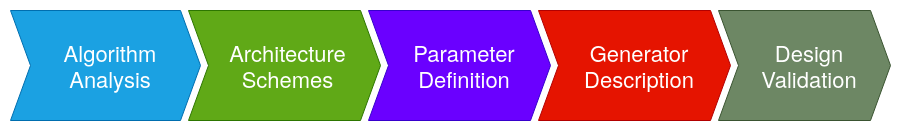
\includegraphics[width=1.0\textwidth]{Figures/Methodology-metadesign}
        \caption{Méthodologie de méta conception}
        \label{ch.resume:sec.exploration:fig.metadesign}
    \end{figure}

    Dans un deuxième temps, nous nous intéressons au processus d'exploration de ces espaces de conception, et proposons la {\bf méta exploration}, une méthodologie d'exploration qui se basent sur la {\bf méta conception}.
    Cette méthodologie repose encore une fois sur l'expertise des développeurs afin de maximiser la flexibilité et la généricité de l'approche (Fig. \ref{ch.resume:sec.exploration:fig.metaexploration}).
    Nous discutons de l'utilisation du paradigme de programmation fonctionnelle\footnote{Chisel étant un langage basé sur scala, proposant donc des fonctionnalités de programmation fonctionnelle} pour la définition des stratégies d'exploration d'espace de conception.
    Plus précisément, nous nous intéressons à une sous classe des stratégies d'exploration, les stratégies séquentielles, et proposons d'utiliser ce paradigme de programmation pour capturer la nature même de composition de ces stratégies.
    Ainsi, nous proposons de considérer les stratégies d'exploration comme une composition d'étapes basiques qui opèrent sur des espaces de conception, et qui peuvent dont être composées pour construire des stratégies plus complexes.
    Chaque stratégie basique repose à la fois sur les métriques d'intérêt à considérer, sur la façon à utiliser pour les estimer et sur comment comparer les différentes implémentations de l'espace de façon efficace (cela peut reposer sur une comparaison exhaustive de toutes les implémentations afin d'optimiser les critères d'intérêt, mais aussi sur des heuristiques moins complexes afin de réduire la durée des processus d'exploration produits ainsi).

    \begin{figure}[h!]
        \centering
        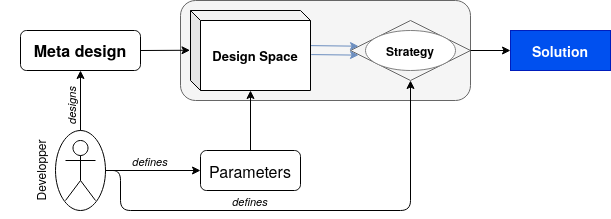
\includegraphics[width=1.0\textwidth]{Figures/Methodology-metaexploration}
        \caption{Méthodologie de méta exploration}
        \label{ch.resume:sec.exploration:fig.metaexploration}
    \end{figure}

    Une formalisation mathématique de cette approche est proposée, afin de faire le lien entre la théorie méthodologique et l'utilisation de la programmation fonctionnelle pour l'implémenter, et plusieurs stratégies basiques sont définies comme preuves de concept.
    Parmi elles, des méthodes classiques d'opération sur des collections (les collections étant ici les espaces de conception à explorer) sont introduites, à savoir les méthodes {\it map} (application exhaustive d'une fonction sur l'ensemble des implémentations qui composent un espace), {\it sort} (un tri de l'espace basé sur l'application d'estimateurs sur l'ensemble des implémentations et sur une relation d'ordre explicite) et {\it prune} (un élagage de l'espace, lui aussi basé sur l'application exhaustive d'une fonction binaire qui défini quelles implémentations doivent être retirées de l'espace de conception, et quelles implémentations doivent rester).
    Nous proposons également deux stratégies plus complexes, basées sur une exploration des voisinages directs des implémentations dans les espaces de conception, afin d’accélérer les processus d'exploration pour les cas d'utilisation où une application exhaustive est infaisable dans un temps raisonnable
    Ces stratégies peuvent donc être utilisées pour réaliser respectivement un tri rapide et un élagage rapide des espaces de conception.

    Dans ce chapitre, nous proposons donc une méthodologie duale d'exploration d'espace de conception qui repose sur l'utilisation de l'expertise des développeurs matériel, permettant de définir des processus d'exploration flexibles et paramétrables, reposant sur la programmation fonctionnelle afin de maximiser l'expressivité des utilisateurs.

\section{Expérimentations et résultats}
\label{ch.resume:sec.expe}
    Afin de démontrer l'utilisabilité de la méthodologie d'exploration d'espace de conception présentée dans les chapitres précédents, un démonstrateur logiciel nommé {\bf QECE} ({\it Quick Exploration using Chisel Estimators}) est proposé dans ce chapitre.
    De plus, la structure interne du logiciel ainsi que les détails intéressants d'implémentation sont décrits pour permettre aux utilisateurs de mieux appréhender les possibilités qu'un tel outil peut apporter au monde de la conception numérique.

    Toujours dans le but de démontrer l'utilisabilité de la méthodologie proposée, un banc d'applications représentatives de l'utilisation des FPGAs en tant que dispositifs d'accélération matérielle est proposé.
    Chaque noyau applicatif composant ce banc a été développé en appliquant la méthodologie de {\bf méta conception}, les détails d'implémentations pouvant être trouvés en annexe du manuscrit en langue anglaise.
    Des expérimentations d'estimation et d'exploration ont été menées sur trois noyaux de ce banc ({\it GEMM}, un algorithme de multiplication de matrices, {\it FFT}, un algorithme provenant du monde du traitement du signal, et {\it Black Scholes}, un modèle de calcul de la valeur d'une action basé sur la méthode de Monte Carlo), afin de mesurer la qualité des estimateurs introduits en Section \ref{ch.resume:sec.estimation}, mais aussi des stratégies d'exploration proposées en Section \ref{ch.resume:sec.exploration}.

    Tout d'abord, nous quantifions l'erreur introduite par les différents estimateurs, démontrant que la méthodologie d'estimation de la consommation des ressources basée sur l'analyse de la représentation intermédiaire introduit une erreur importante par rapport aux résultats des logiciels de synthèses, mais que les métriques estimées peuvent tout de même être utilisée pour inférer la qualité des implémentations considérées en première approche.
    En revanche, nous démontrons que la méthodologie d'estimation des chemins critiques des circuits, basée elle aussi sur une analyse de la représentation intermédiaire, produit des résultats très éloignés de la réalité (à savoir, les résultats du logiciel de synthèse logique), très peu fiables, et en un temps qui peut être plus élévé que les outils propriétaires que l'on cherche à approximer.
    De ce fait, cette approche est laissée de côté comme piste d'amélioration du logiciel proposé, et les estimations de chemins critiques et de fréquences maximale d'opération utilisées dans la suite de nos travaux sont basées sur l'analyse des rapports des outils de synthèse logiques, bien plus fiables mais pouvant être coûteux en temps et en ressources de calcul.
    Enfin, nous démontrons l'utilisabilité de la méthodologie empirique d'estimation de la qualité de service des circuits sur un exemple simple (calcul d'un produit scalaire), afin de montrer comment l'instrumentation des différents moteurs de simulation disponibles dans le flot de conception Chisel peuvent permettre d'estimer des métriques intéressantes, pour certains cas d'utilisation.

    Après avoir abordé l'aspect qualitatif des différents estimateurs proposés, et démontré leurs utilisabilités, nous nous intéressons maintenant à démontrer l'intérêt de l'approche fonctionnelle pour résoudre le problème de l'exploration d'espace de conception, en proposant et en comparant différentes stratégies de {\bf méta exploration} comme définies dans le Section \ref{ch.resume:sec.exploration}.
    Tout d'abord, nous comparons trois stratégies d'exploration sur le noyau applicatif {\it GEMM}, démontrons qu'une approche basée sur l'utilisation de l'expertise du développeur peut permettre de réduire d'un facteur 4 le temps passé pour explorer un espace restreint (42 implémentations) de façon efficace, comparé à une solution par "force brute" consistant à synthétiser toutes les implémentations disponibles.
    Nous démontrons ensuite, sur le noyau applicatif de Transformée de Fourier Rapide ({\it FFT}), qu'une des limites de cette approche d'exploration est la possibilité d'exprimer des relations d'ordres claires entre les implémentations qui composent l'espace de conception, c'est à dire utiliser les métriques d'intérêts disponibles pour définir comparer la qualité des implémentations dans un cas d'utilisation donné.
    Sans modèle applicatif adéquat, il est impossible de comparer, par exemple, des noyaux qui considèrent différentes tailles d'élements dans les calculs, puisque des éléments plus grands vont augmenter la qualité de service des circuits générés, mais également la consommation de ressources --- c'est donc au développeur de spécifier exactement cette relation d'ordre, qui ne peut être implicite.
    Ainsi, sur ce noyau applicatif, nous démontrons que les stratégies avancées d'exploration peuvent s'avérer moins performantes (en terme de temps) que la stratégie par "force brute", dans le cas où le modèle applicatif fourni est trop faible pour exposer des espaces de conceptions suffisamment large pour bénéficier de cette approche.
   Enfin, et pour palier ce problème, nous proposons une stratégie d'exploration de l'espace de conception des noyaux {\it Black Scholes}, basée sur une approche en deux temps: tout d'abord, l'utilisation d'une approche empirique pour estimer la qualité de service (l'erreur introduite par l'implémentation matérielle par rapport à une référence logicielle) et discriminer toutes les implémentations qui introduisent une erreur trop importante, avant de parcourir les implémentations restantes pour sélectionner celle qui proposent le meilleur débit possible, pour la carte FPGA cible. 
    Une telle stratégie peut être définie en une dizaine de ligne dans le logiciel {\bf QECE}, démontrons à la fois l'intérêt et la concision de l'approche fonctionnelle pour l'exploration d'espace de conception.

    Dans ce chapitre, nous démontrons l'utilisabilité de la méthodologie de {\bf méta exploration}, contribution principale de cette thèse, à travers l'usage d'un logiciel démonstrateur ({\bf QECE}) que nous avons développé, et de multiples expérimentations sur des noyaux applicatifs également développés par nos soins.
    L'accent est mis sur l'utilisation de l'expertise des développeurs matériels pour proposer des stratégies intelligentes qui convergent rapidement pour les cas d'utilisation considérés.

\section{Conclusion}
\label{ch.resume:sec.conclusion}
    Dans ce travail de thèse, nous nous intéressons au paradigme émergent des langages de construction matérielle, dont Chisel est un exemple, afin d'améliorer la productivité des développeurs matériel.
    Plus précisément, nous proposons une approche originale pour résoudre le problème de l'exploration d'espace de conception, qui se base sur une méthodologie innovante de conception couplée à l'utilisation du paradigme de programmation fonctionnelle afin de définir des stratégies d'exploration intelligentes, car définies par les développeurs eux mêmes.

    Nous démontrons l'utilisabilité d'une telle méthodologie à l'aide d'un logiciel développeur, nommé {\bf QECE}, que nous avons développé pour l'occasion, qui propose une bibliothèque de méthodologies d'estimation de métriques d'intérêt pour les circuits considérés, et une bibliothèque de stratégies basiques d'exploration qui peuvent être composées pour construire des stratégies plus complexes et adaptables aux différents cas d'utilisation.
    Cette approche permet une grande flexibilité d'utilisation, afin d'être réutilisable et adaptable à de nouveaux cas d'utilisation, améliorant ainsi la productivité des concepteurs numériques.

%%%%%%%%%%%%%%%%%%%%%%%%%%%%%%%%%%%%%%%%%%%%%%%%%%%%%%%%%%%%%%%%%%%%%%%%%%%%%%%%%
%%%%%%%%%%%%%%%%%%%%%%%%%%%%%%%%%%%%%%%%%%%%%%%%%%%%%%%%%%%%%%%%%%%%%%%%%%%%%%%
